\begin{center}
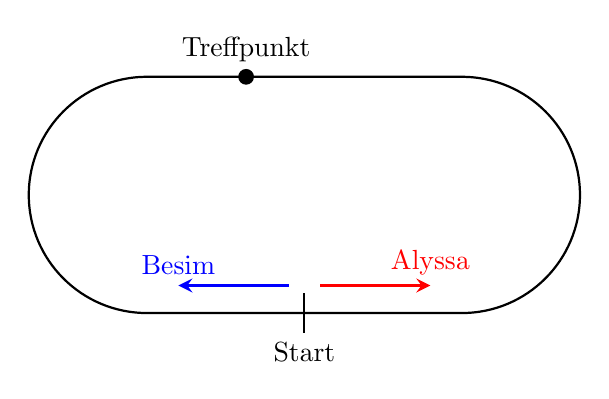
\begin{tikzpicture}[>=stealth]
 \draw[thick] (-2,-1.5) -- (2,-1.5) arc (-90:90:1.5) -- (-2,1.5) arc (90:270:1.5);
 \draw[thick] (0,-1.75) -- (0,-1.25);
 \node[below] at (0,-1.75) {Start};
 \draw[->, very thick, red] (0.2,-1.15) -- (1.6,-1.15) node[above] {Alyssa};
 \draw[->, very thick, blue] (-0.2,-1.15) -- (-1.6,-1.15) node[above] {Besim};
 \fill (-0.74,1.5) circle (0.1) node[above=2pt] {Treffpunkt};
\end{tikzpicture}
\end{center}

Bis zum Kreuzen legen die beiden zusammen genau eine Runde zurück:
\begin{align}
 v_\mathrm{A}\,t + v_\mathrm{B}\,t &= s
\end{align}
Sie kreuzen sich deshalb nach
\begin{align}
 t &= \tKF = \frac{\sB}{\vAl+\vBe} = \tK \approx \result{\tKP{0}{2}}
\end{align}
Alyssa hat dann die Strecke
\begin{align}
 s_\mathrm{A} &= v_\mathrm{A}\,t = \sAlF = \sAl \approx \result{\sAlP{0}{3}}
\end{align}
zurückgelegt; der Treffpunkt liegt also \sAlP{0}{3} vom Start entfernt in Alyssas Laufrichtung, oder $s_\mathrm{B} = \sBeP{0}{3}$ vom Start in Besims Laufrichtung.
